%------------------------------------------------
\section{Problem}
%------------------------------------------------

\begin{frame}
\frametitle{Problem description}
The problem consists in \emph{scheduling a set of job}, on a set of \emph{unrelated parallel machines}, while optimizing objective functions.

\medskip

%Each job has a \emph{release date} (hard constraint), a \textbf{due date} (soft constraint), and a \emph{weighted penalty cost} depending on the generete delay after its due date.

Job characteristics are: 
\begin{itemize}
	\item \emph{release date} (hard constraint)
	\item \emph{due date} (soft constraint)
	\item \emph{weighted penalty cost}%, depending on the generated delay after due date.
\end{itemize}

\medskip

Each job have to be processed by only one machine, selected from a set of eligible ones, where \emph{processing time} and \emph{energy consumption} depend by the selected machine.

\medskip

In order to process a job the machines must be setup and this setup time depends on the \emph{machine} and the \emph{previously scheduled job} on it.

\begin{displaymath}
R_m | M_j,p_{ij},E_{ij},r_j,d_j,w_j,s_{ijk} | \displaystyle\sum w_j T_j, \displaystyle\sum E_{ij}, \displaystyle\sum S_{ijk}
\end{displaymath}

\end{frame}


\begin{frame} \frametitle{Problem example}
\begin{figure}[t]
	\label{fig:example_sched}
	\centering
	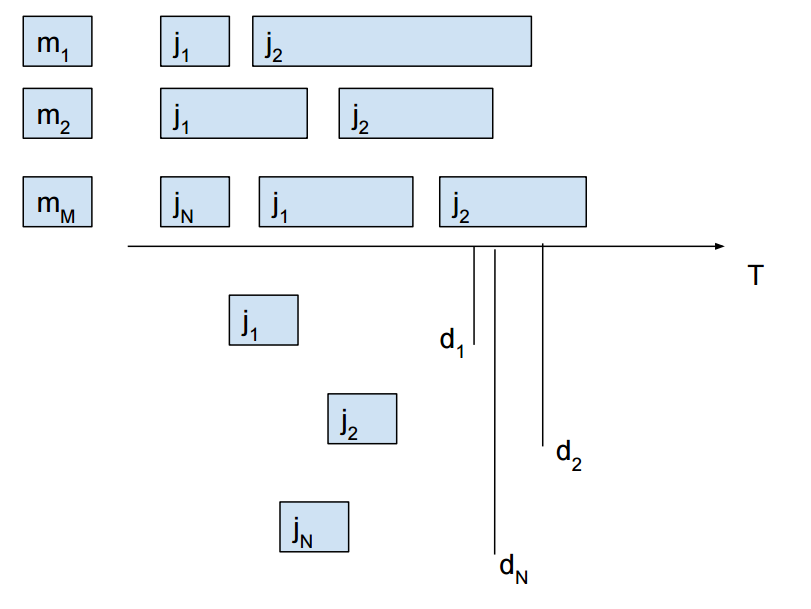
\includegraphics[width=.75\columnwidth]{example_sched}
	\caption{Scheduling example 1}
\end{figure}
\end{frame}

\begin{frame} \frametitle{Problem example}
\begin{figure}[t]
	\label{fig:example_sched2}
	\centering
	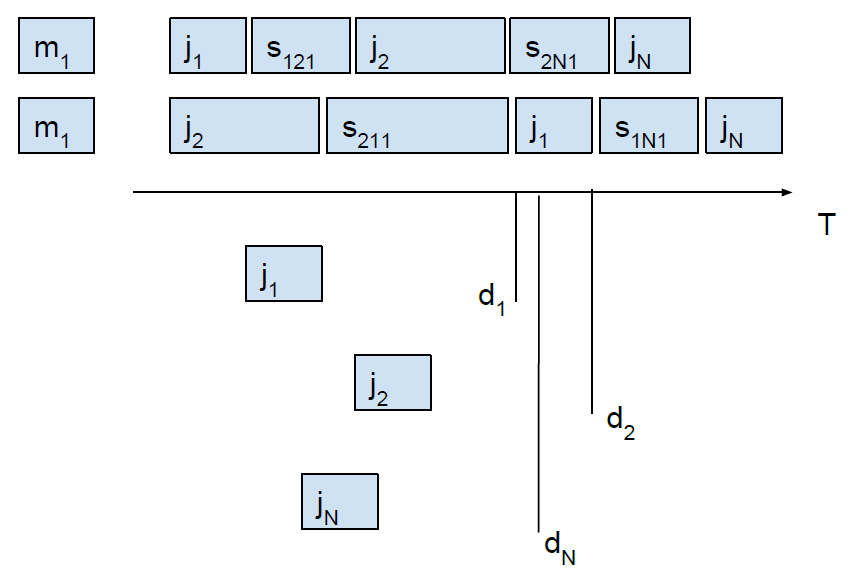
\includegraphics[width=.75\columnwidth]{example_sched2}
	\caption{Scheduling example 2}
\end{figure}
\end{frame}

\begin{frame} \frametitle{Problem objectives}
In relation to a possible scheduling solution $s$, three different objective functions can be stated:
\begin{itemize}
\item $TT(s)$: total weighted tardiness of the jobs,
\item $EN(s)$: energy consumption,
\item $ST(s)$: total setup time.
\end{itemize} 
The aim is to simultaneously optimized them in a multi-objective function:
\begin{equation}
\label{eq_1:multi_objective_function}
s^* = \operatorname*{arg\,min}_{s \in S} [TT(s),EN(s),ST(s)] 
\end{equation}
where $S$ denotes the feasibility space for the problem solutions.

\end{frame}


\begin{frame}
\frametitle{Problem objectives}

The three objective functions in (\ref{eq_1:multi_objective_function}) are aggregated into a scalar normalized objective function F:
\begin{equation}
\label{eq_2:normalized_multi_objective_function}
F(s) = \displaystyle\sum_{g=1}^{3} \Pi_{g} \cdot \frac{f_g(s) - f^{-}_{g}}{f^{+}_{g} - f^{-}_{g}}
\end{equation}
where:
\begin{itemize}
\item $f_g(s)$,~$g\in\{1,2,3\}$, represents $TT(s)$, $EN(s)$ and $ST(s)$.

\item $f^{-}_{g}$ represents the best (\emph{minimum}) value %for the $g$-th component when it is optimized individually
\item $f^{+}_{g}$ is an estimation of the worse value for $f_{g}(s)$%, that can be fixed as $f^{+}_{g} = \operatorname*{max}_{h\neq g} f_{g}(s_{h}^{*})$%, where $(s_{h}^{*})$ is the optimal solution found when the objective $f_{h}(s)$ is individually optimized
\item $\Pi_{g}$,~$g\in\{1,2,3\}$, represents the relative importance given by the decision maker to the different objective, where $\sum_{g}\Pi_{g} = 1$
\end{itemize}

\end{frame}